Este capítulo descreve, de forma sistemática, os procedimentos adotados para a construção,
treinamento e avaliação dos modelos considerados neste trabalho. Em particular, são detalhados
os processos de particionamento dos dados, seleção de hiperparâmetros e geração de dados
experimentais, seguindo práticas consolidadas na literatura de aprendizado de máquina aplicado
à análise de sobrevivência.

\section{Recursos Computacionais}

\noindent Nesta seção, são apresentados os principais recursos computacionais utilizados no
desenvolvimento deste trabalho, incluindo ferramentas para escrita do documento,
linguagens de programação empregadas na implementação dos modelos e bibliotecas utilizadas
na resolução dos problemas de otimização convexa. A escolha dessas ferramentas foi guiada
pela necessidade de garantir rigor científico, reprodutibilidade dos experimentos e
eficiência computacional na implementação dos algoritmos propostos.

\subsection{Ambiente de desenvolvimento e escrita}

A redação deste trabalho foi realizada utilizando o sistema de preparação de documentos
\LaTeX, amplamente adotado na comunidade científica devido à sua capacidade de lidar de
forma robusta com expressões matemáticas, referências bibliográficas e formatação de
documentos técnicos. O uso do \LaTeX\ foi particularmente importante neste trabalho,
dado o elevado número de equações e demonstrações envolvidas na formulação dos modelos
baseados em máquinas de vetores de suporte.

Para a edição do código-fonte e do documento, foi utilizado o editor Visual Studio Code
(VSCode), que oferece um ambiente leve e altamente configurável. O VSCode permite integração
com diversas extensões, possibilitando suporte eficiente tanto para a escrita em \LaTeX\
quanto para o desenvolvimento em linguagens de programação como Python. Entre as
funcionalidades utilizadas, destacam-se a navegação facilitada entre arquivos,
realce de sintaxe, execução de scripts e integração com sistemas de controle de versão.

\subsection{Linguagem de programação e implementação dos modelos}

A implementação dos modelos propostos neste trabalho foi realizada na linguagem de
programação Python, devido à sua ampla adoção na área de ciência de dados e aprendizado
de máquina, bem como à disponibilidade de bibliotecas eficientes para computação numérica.

O Python foi utilizado tanto para a geração de dados simulados quanto para a implementação
do algoritmo proposto, o GG-KM. As bibliotecas utilizadas para estimação do modelo foram NumPy \cite{harris2020array},
que oferece estruturas eficientes para operações matriciais e vetoriais, e o SciPy \cite{virtanen2020scipy}, que contém
diferentes métodos de otimização, como, por exemplo, o L-BFGS.

% Além disso, o Python permite uma integração natural com bibliotecas de otimização e
% facilita a prototipagem de modelos matemáticos complexos, o que foi essencial para o
% desenvolvimento e validação das abordagens propostas neste trabalho.

% \subsection{Otimização convexa}

% A resolução dos problemas de otimização associados aos modelos SVCR e WSVCR foi realizada
% por meio da biblioteca CVXOPT, uma biblioteca especializada em programação convexa
% desenvolvida para a linguagem Python.

% A escolha do CVXOPT deve-se ao fato de que os problemas dual dos modelos baseados em
% máquinas de vetores de suporte podem ser formulados como problemas de programação
% quadrática convexa. Nesse contexto, o CVXOPT fornece rotinas eficientes e numericamente
% estáveis para a obtenção da solução ótima global, garantindo a correta resolução do
% problema sem a necessidade de implementação manual de algoritmos iterativos, como o
% Sequential Minimal Optimization (SMO).

% O uso de uma biblioteca consolidada como o CVXOPT também contribui para a reprodutibilidade
% dos resultados, uma vez que os algoritmos de otimização empregados são amplamente testados
% e documentados na literatura.


\section{Particionamento dos dados}

A avaliação do desempenho preditivo dos modelos foi conduzida por meio de um esquema de
validação baseado na divisão dos dados em conjuntos de treinamento e teste. Especificamente,
adotou-se uma estratégia de holdout, na qual $70\%$ das observações foram utilizadas para
treinamento e os $30\%$ restantes reservados para teste.

A separação foi realizada de forma aleatória, preservando, sempre que aplicável, a estrutura
dos dados censurados, de modo a garantir que ambos os subconjuntos apresentassem proporções
semelhantes de observações censuradas e não censuradas. Essa precaução é particularmente
importante em problemas de análise de sobrevivência, uma vez que a distribuição dos tipos de
censura pode influenciar significativamente o desempenho dos modelos.

Adicionalmente, com o objetivo de reduzir a variabilidade associada a uma única partição,
o procedimento de holdout foi repetido múltiplas vezes. As métricas de desempenho foram então agregadas ao longo dessas
repetições, considerando medidas como média, mediana e desvio padrão, proporcionando uma
avaliação mais robusta e estável.

\section{Estudo de simulação e Métricas de Erro}

Com o objetivo de avaliar o desempenho do modelo GG-KM em diferentes cenários de complexidade da fração
de cura, foi conduzido um estudo de simulação, seguindo a mesma estrutura de geração
de dados proposta por \citeonline{pal2023semiparametric}, adaptada ao contexto do modelo de tempo de promoção.

Foram considerados dois tamanhos de amostra, $n=300$ e $n=600$. Em cada replicação, os dados foram
particionados em conjunto de treinamento e teste, sendo dois terços das observações destinados ao
treinamento e o terço restante utilizado para avaliação preditiva.

Cada conjunto de dados foi gerado a partir de duas covariáveis independentes,
\[
x_1,x_2 \sim N(0,1).
\]

A estrutura de cura foi construída a partir de três métodos distintos para a geração da probabilidade
de não cura, permitindo avaliar o comportamento do modelo sob diferentes graus de linearidade e não
linearidade. Para o primeiro caso, considera-se uma fronteira linear, dada por
\[
\pi(\mathbf{x})
=
\frac{\exp(0.3-5x_1-3x_2)}
{1+\exp(0.3-5x_1-3x_2)}.
\]

Esse cenário representa a estrutura clássica de regressão logística, em que indivíduos curados e não curados são linearmente separáveis.

No segundo método, é introduzido uma relação quadrática entre as covariáveis, com o objetivo de avaliar a capacidade
do modelo em capturar superfícies de decisão não lineares. Portanto, tem-se:
\[
\pi(\mathbf{x})
=
\frac{\exp(0.3+5x_1^2-3x_2^2)}
{1+\exp(0.3+5x_1^2-3x_2^2)}.
\]

Por fim, o para o terceiro método, é considerado uma estrutura não linear e periódica:
\[
\pi(\mathbf{x})
=
\exp\left\{-\exp(0.3-5\cos(x_1)-3\sin(x_2))\right\}.
\]

\begin{figure}[htb]
    \centering
    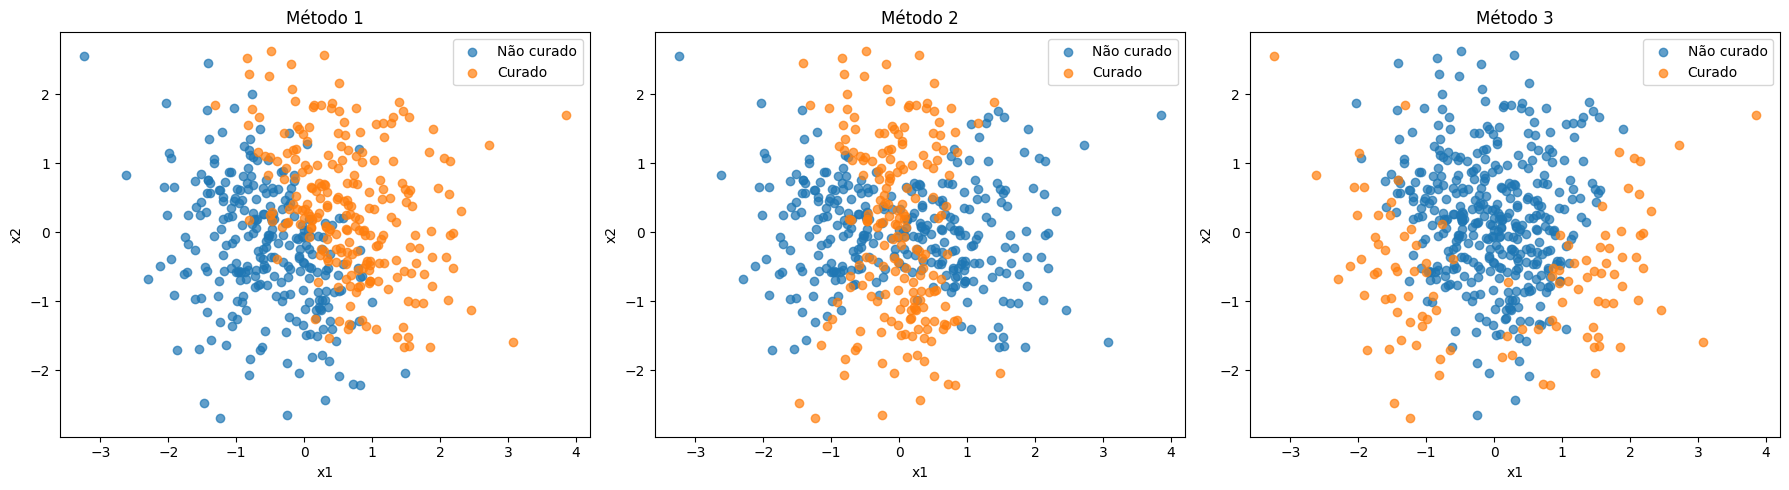
\includegraphics[width=1\textwidth]{images/plot_metodos123.png}
    \caption{Simulação de curados e não curados sobre os três métodos descritos. Respectivamente, pode-se observar o método 1, 2 e 3.}
    \label{fig:exemplo_metodo}
\end{figure}

Esse cenário impõe fronteiras de classificação complexas, sendo particularmente útil para avaliar a
flexibilidade da abordagem baseada em kernels. Os dados simulados, considerando cada um dos três casos, pode
ser visualizado na Figura~\ref{fig:exemplo_metodo}.

Para a componente de latência, os tempos associados aos riscos latentes foram gerados a partir de uma distribuição Weibull, cuja função de risco é dada por
\[
h(t|\mathbf{x})
=
h_0(t)\exp(\beta_1x_1+\beta_2x_2),
\]
onde a função de risco basal foi definida como
\[
h_0(t)=\alpha t^{\alpha-1}, \quad \alpha>0.
\]

Essa especificação implica que os tempos latentes seguem uma distribuição Weibull com parâmetro de forma $\alpha$ e parâmetro de escala

\[
\lambda(\mathbf{x})
=
\left\{
\exp(\beta_1x_1+\beta_2x_2)
\right\}^{-1/\alpha}.
\]

Os valores utilizados para os parâmetros foram $(\alpha,\beta_1,\beta_2)=(2,1,0.5)$ Os tempos de censura
foram gerados independentemente a partir de uma distribuição exponencial com taxa igual a $0.2$, isto é
$C_i \sim \text{Exp}(0.2)$. A partir desta configuração, a proporção de censura obtida para o método 1, 2 e 3
é de aproximadamente 0,60, 0,50 e 0,40, respectivamente. Para a proporção de cura foi obtido aproximadamente 0,50, 0,60 e 0,20.

A geração dos dados simulados foi realizada com base na estrutura do modelo de fração de cura em tempo de
promoção. Nesse contexto, cada indivíduo pode pertencer a um de dois grupos: curados ou suscetíveis ao
evento de interesse. A probabilidade de um indivíduo ser suscetível é dada por $\pi(\mathbf{x}_i)$, enquanto
a probabilidade de ser curado é $1-\pi(\mathbf{x}_i)$.

O processo de simulação ocorre em duas etapas. Inicialmente, para cada indivíduo, gera-se uma variável
uniforme $U_i$ e um tempo de censura $C_i$. O valor de $U_i$ é utilizado para determinar se o indivíduo
pertence ao grupo curado ou suscetível. Caso $U_i \leq 1-\pi(\mathbf{x}_i)$, o indivíduo é classificado como
curado e seu tempo observado corresponde apenas ao tempo de censura.

Por outro lado, se $U_i > 1-\pi(\mathbf{x}_i)$, o indivíduo é considerado suscetível. Nesse caso, gera-se um
tempo latente de falha $Y_i$ utilizando o método da transformada inversa aplicado à função de sobrevivência
populacional. Para isso, sorteia-se uma nova variável uniforme no intervalo $(1-\pi(\mathbf{x}_i),1)$ e
resolve-se a equação associada à função de sobrevivência, obtendo assim o tempo de falha latente.

Por fim, o tempo observado é definido como o mínimo entre o tempo latente de falha e o tempo de censura. O
indicador de falha é então determinado de acordo com qual desses tempos ocorreu primeiro. Esse procedimento garante
que os dados simulados preservem simultaneamente a estrutura de fração de cura e a presença de censura à direita.
O algoritmo pode ser visualizado no Algoritmo~\ref{alg:data_generation}

\begin{algorithm}[H]
\caption{Geração de dados simulados com fração de cura}
\label{alg:data_generation}
\begin{algorithmic}[1]
\For{$i=1,\ldots,n$}
    \State Gerar $U_i \sim \text{Uniform}(0,1)$
    \State Gerar $C_i \sim \text{Exp}(0.2)$

    \If{$U_i \leq 1-\pi(\mathbf{x}_i)$}
        \State Definir $t_i \leftarrow C_i$
        \State Definir $\delta_i \leftarrow 0$
    \Else
        \State Gerar $U_i^* \sim \text{Uniform}(1-\pi(\mathbf{x}_i),1)$
        \State Resolver

        \[
        (1-\pi(\mathbf{x}_i))^{F(Y_i|\mathbf{x}_i)}=U_i^*
        \]
        \State Obter
        \[
        Y_i=
        F^{-1}
        \left(
        \frac{\log(U_i^*)}
        {\log(1-\pi(\mathbf{x}_i))}
        \right)
        \]
        \State Definir $t_i \leftarrow \min(Y_i,C_i)$

        \If{$t_i=Y_i$}
            \State Definir $\delta_i \leftarrow 1$
        \Else
            \State Definir $\delta_i \leftarrow 0$
        \EndIf
    \EndIf
\EndFor
\end{algorithmic}
\end{algorithm}

% A geração dos dados de sobrevivência foi realizada para cada indivíduo $i$ segundo o seguinte algoritmo:

% \begin{enumerate}
%     \item Gerar $U_i \sim \text{Uniform}(0,1)$ e $C_i \sim \text{Exp}(0.2)$;

%     \item Se $U_i \leq 1-\pi(\mathbf{x}_i)$, o indivíduo é considerado curado, definindo-se
%     \[
%     t_i=C_i
%     \quad\text{e}\quad
%     \delta_i=0.
%     \]

%     \item Se $U_i > 1-\pi(\mathbf{x}_i)$, o indivíduo é suscetível:
%     \begin{enumerate}
%         \item Gerar $U_i^* \sim \text{Uniform}(1-\pi(\mathbf{x}_i),1)$;

%         \item Obter o tempo latente $Y_i$ resolvendo
%         \[
%         (1-\pi(\mathbf{x}_i))F(Y_i|\mathbf{x}_i)=U_i^*,
%         \]

%         ou equivalentemente,

%         \[
%         Y_i=
%         F^{-1}
%         \left(
%         \frac{\log(U_i^*)}
%         {\log(1-\pi(\mathbf{x}_i))}
%         \right);
%         \]

%         \item Definir o tempo observado:
%         \[
%         t_i=\min(Y_i,C_i);
%         \]

%         \item Definir o indicador de falha:
%         \[
%         \delta_i=
%         \begin{cases}
%         1, & \text{se } t_i=Y_i,\\
%         0, & \text{caso contrário.}
%         \end{cases}
%         \]
%     \end{enumerate}
% \end{enumerate}

O desempenho do modelo GG-KM foi avaliado com base no viés, erro quadrático médio (EQM) e no \textit{Integrated Brier Score} (IBS) com ajuste IPCW (\textit{Inverse Probability of Censoring Weighting}) \cite{dong2020inverse}, permitindo mensurar tanto a qualidade da estimação dos parâmetros quanto a capacidade preditiva do modelo.

Seja $\hat{S}_i(t)$ a probabilidade de sobrevivência estimada para o indivíduo $i$ no tempo $t$, e $T_i^*$ o tempo observado. Os pesos IPCW são definidos por

\[
\omega_i(t)=
\frac{\mathbb{I}(T_i^*\leq t,\delta_i=1)}{\hat{G}(T_i^*)}
+
\frac{\mathbb{I}(T_i^*>t)}{\hat{G}(t)},
\]

em que $\hat{G}(t)$ representa a função de sobrevivência do mecanismo de censura, geralmente estimada pelo método de Kaplan-Meier.

Com isso, o Brier Score ajustado por IPCW no tempo $t$ é dado por

\[
BS_{IPCW}(t)
=
\frac{1}{\tilde{n}(t)}
\sum_{i=1}^{n}
\left[
\hat{S}_i(t)^2
\frac{\mathbb{I}(T_i^*\leq t,\delta_i=1)}{\hat{G}(T_i^*)}
+
(1-\hat{S}_i(t))^2
\frac{\mathbb{I}(T_i^*>t)}{\hat{G}(t)}
\right],
\]
em que
\[
\tilde{n}(t)=\sum_{i=1}^{n}\omega_i(t)
\]
corresponde à soma dos pesos IPCW no tempo $t$.


O IBS é então definido como a integral do Brier Score ao longo do intervalo de acompanhamento:
\[
IBS=
\frac{1}{\tau}
\int_0^\tau BS_{IPCW}(t)\,dt,
\]
em que $\tau$ representa o tempo máximo de observação.

Por fim, a estimativa do EQM e do viés em relação à probabilidade dos não curados foi obtida a partir das seguintes expressões, respectivamente \cite{pal2023semiparametric}:

$$
\text{Viés}\left(\widehat{\pi}\left(\mathbf{x}\right)\right) =
\frac{1}{N_1} \sum_{r=1}^{N_1} \left[\frac{1}{n}\sum_{i=1}^{n}\{\hat{\pi^{\left(r\right)}}\left(\mathbf{x}_i\right) -
\pi^{\left(r\right)}\left(\mathbf{x}_i\right)\}\right]\text{,}
$$

$$
\text{EQM}\left(\widehat{\pi}\left(\mathbf{x}\right)\right) = \frac{1}{N_1} \sum_{r=1}^{N_1} \left[\frac{1}{n}\sum_{i=1}^{n}\left\{\hat{\pi^{\left(r\right)}}\left(\mathbf{x}_i\right) - \pi^{\left(r\right)}\left(\mathbf{x}_i\right)\right\}^2\right]\text{.}
$$


% Este capítulo descreve, de forma sistemática, os procedimentos adotados para a construção,
% treinamento e avaliação dos modelos considerados neste trabalho. Em particular, são detalhados
% os processos de particionamento dos dados, seleção de hiperparâmetros e geração de dados
% experimentais, seguindo práticas consolidadas na literatura de aprendizado de máquina aplicado
% à análise de sobrevivência.

% \section{Particionamento dos dados}

% A avaliação do desempenho preditivo dos modelos foi conduzida por meio de um esquema de
% validação baseado na divisão dos dados em conjuntos de treinamento e teste. Especificamente,
% adotou-se uma estratégia de holdout, na qual $70\%$ das observações foram utilizadas para
% treinamento e os $30\%$ restantes reservados para teste.

% A separação foi realizada de forma aleatória, preservando, sempre que aplicável, a estrutura
% dos dados censurados, de modo a garantir que ambos os subconjuntos apresentassem proporções
% semelhantes de observações censuradas e não censuradas. Essa precaução é particularmente
% importante em problemas de análise de sobrevivência, uma vez que a distribuição dos tipos de
% censura pode influenciar significativamente o desempenho dos modelos.

% Adicionalmente, com o objetivo de reduzir a variabilidade associada a uma única partição,
% o procedimento de holdout foi repetido múltiplas vezes. As métricas de desempenho foram então agregadas ao longo dessas
% repetições, considerando medidas como média, mediana e desvio padrão, proporcionando uma
% avaliação mais robusta e estável.

% \section{Estudo de simulação e Métricas de Erro}

% Com o objetivo de avaliar o desempenho do modelo GG-KM em diferentes cenários de complexidade da fração
% de cura, foi conduzido um estudo de simulação, seguindo a mesma estrutura de geração
% de dados proposta por \citeonline{pal2023semiparametric}, adaptada ao contexto do modelo de tempo de promoção.

% Foram considerados dois tamanhos de amostra, $n=300$ e $n=600$. Em cada replicação, os dados foram
% particionados em conjunto de treinamento e teste, sendo dois terços das observações destinados ao
% treinamento e o terço restante utilizado para avaliação preditiva.

% Cada conjunto de dados foi gerado a partir de duas covariáveis independentes,
% \[
% x_1,x_2 \sim N(0,1).
% \]

% A estrutura de cura foi construída a partir de três métodos distintos para a geração da probabilidade
% de não cura, permitindo avaliar o comportamento do modelo sob diferentes graus de linearidade e não
% linearidade. Para o primeiro caso, considera-se uma fronteira linear, dada por
% \[
% \pi(\mathbf{x})
% =
% \frac{\exp(0.3-5x_1-3x_2)}
% {1+\exp(0.3-5x_1-3x_2)}.
% \]

% Esse cenário representa a estrutura clássica de regressão logística, em que indivíduos curados e não curados são linearmente separáveis.

% No segundo método, é introduzido uma relação quadrática entre as covariáveis, com o objetivo de avaliar a capacidade
% do modelo em capturar superfícies de decisão não lineares. Portanto, tem-se:
% \[
% \pi(\mathbf{x})
% =
% \frac{\exp(0.3+5x_1^2-3x_2^2)}
% {1+\exp(0.3+5x_1^2-3x_2^2)}.
% \]

% Por fim, o para o terceiro método, é considerado uma estrutura não linear e periódica:
% \[
% \pi(\mathbf{x})
% =
% \exp\left\{-\exp(0.3-5\cos(x_1)-3\sin(x_2))\right\}.
% \]

% \begin{figure}[htb]
%     \centering
%     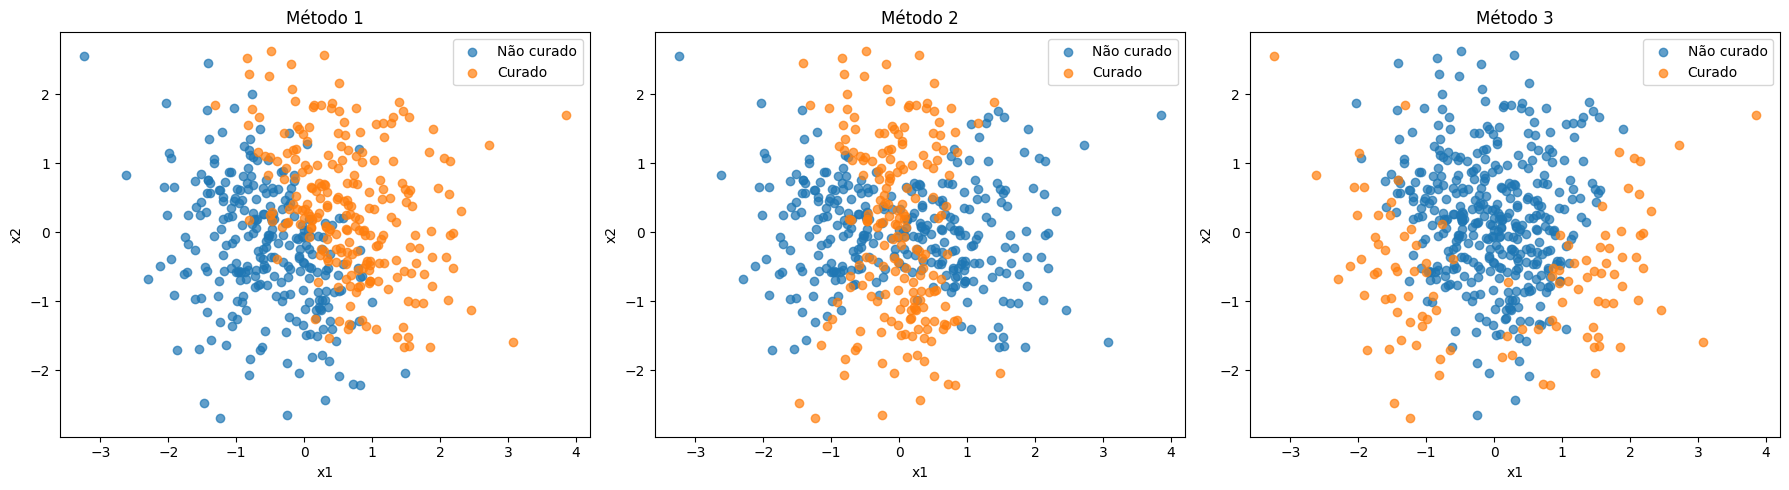
\includegraphics[width=1\textwidth]{images/plot_metodos123.png}
%     \caption{Simulação de curados e não curados sobre os três métodos descritos. Respectivamente, pode-se observar o método 1, 2 e 3.}
%     \label{fig:exemplo_metodo}
% \end{figure}

% Esse cenário impõe fronteiras de classificação complexas, sendo particularmente útil para avaliar a
% flexibilidade da abordagem baseada em kernels. Os dados simulados, considerando cada um dos três casos, pode
% ser visualizado na Figura~\ref{fig:exemplo_metodo}.

% Para a componente de latência, os tempos associados aos riscos latentes foram gerados a partir de uma distribuição Weibull, cuja função de risco é dada por
% \[
% h(t|\mathbf{x})
% =
% h_0(t)\exp(\beta_1x_1+\beta_2x_2),
% \]
% onde a função de risco basal foi definida como
% \[
% h_0(t)=\alpha t^{\alpha-1}, \quad \alpha>0.
% \]

% Essa especificação implica que os tempos latentes seguem uma distribuição Weibull com parâmetro de forma $\alpha$ e parâmetro de escala

% \[
% \lambda(\mathbf{x})
% =
% \left\{
% \exp(\beta_1x_1+\beta_2x_2)
% \right\}^{-1/\alpha}.
% \]

% Os valores utilizados para os parâmetros foram $(\alpha,\beta_1,\beta_2)=(2,1,0.5)$ Os tempos de censura
% foram gerados independentemente a partir de uma distribuição exponencial com taxa igual a $0.2$, isto é
% $C_i \sim \text{Exp}(0.2)$. A partir desta configuração, a proporção de censura obtida para o método 1, 2 e 3
% é de aproximadamente 0,60, 0,50 e 0,40, respectivamente. Para a proporção de cura foi obtido aproximadamente 0,50, 0,60 e 0,20.

% A geração dos dados simulados foi realizada com base na estrutura do modelo de fração de cura em tempo de
% promoção. Nesse contexto, cada indivíduo pode pertencer a um de dois grupos: curados ou suscetíveis ao
% evento de interesse. A probabilidade de um indivíduo ser suscetível é dada por $\pi(\mathbf{x}_i)$, enquanto
% a probabilidade de ser curado é $1-\pi(\mathbf{x}_i)$.

% O processo de simulação ocorre em duas etapas. Inicialmente, para cada indivíduo, gera-se uma variável
% uniforme $U_i$ e um tempo de censura $C_i$. O valor de $U_i$ é utilizado para determinar se o indivíduo
% pertence ao grupo curado ou suscetível. Caso $U_i \leq 1-\pi(\mathbf{x}_i)$, o indivíduo é classificado como
% curado e seu tempo observado corresponde apenas ao tempo de censura.

% Por outro lado, se $U_i > 1-\pi(\mathbf{x}_i)$, o indivíduo é considerado suscetível. Nesse caso, gera-se um
% tempo latente de falha $Y_i$ utilizando o método da transformada inversa aplicado à função de sobrevivência
% populacional. Para isso, sorteia-se uma nova variável uniforme no intervalo $(1-\pi(\mathbf{x}_i),1)$ e
% resolve-se a equação associada à função de sobrevivência, obtendo assim o tempo de falha latente.

% Por fim, o tempo observado é definido como o mínimo entre o tempo latente de falha e o tempo de censura. O
% indicador de falha é então determinado de acordo com qual desses tempos ocorreu primeiro. Esse procedimento garante
% que os dados simulados preservem simultaneamente a estrutura de fração de cura e a presença de censura à direita.
% O algoritmo pode ser visualizado no Algoritmo~\ref{alg:data_generation}

% \begin{algorithm}[H]
% \caption{Geração de dados simulados com fração de cura}
% \label{alg:data_generation}
% \begin{algorithmic}[1]
% \For{$i=1,\ldots,n$}
%     \State Gerar $U_i \sim \text{Uniform}(0,1)$
%     \State Gerar $C_i \sim \text{Exp}(0.2)$

%     \If{$U_i \leq 1-\pi(\mathbf{x}_i)$}
%         \State Definir $t_i \leftarrow C_i$
%         \State Definir $\delta_i \leftarrow 0$
%     \Else
%         \State Gerar $U_i^* \sim \text{Uniform}(1-\pi(\mathbf{x}_i),1)$
%         \State Resolver

%         \[
%         (1-\pi(\mathbf{x}_i))^{F(Y_i|\mathbf{x}_i)}=U_i^*
%         \]
%         \State Obter
%         \[
%         Y_i=
%         F^{-1}
%         \left(
%         \frac{\log(U_i^*)}
%         {\log(1-\pi(\mathbf{x}_i))}
%         \right)
%         \]
%         \State Definir $t_i \leftarrow \min(Y_i,C_i)$

%         \If{$t_i=Y_i$}
%             \State Definir $\delta_i \leftarrow 1$
%         \Else
%             \State Definir $\delta_i \leftarrow 0$
%         \EndIf
%     \EndIf
% \EndFor
% \end{algorithmic}
% \end{algorithm}

% % A geração dos dados de sobrevivência foi realizada para cada indivíduo $i$ segundo o seguinte algoritmo:

% % \begin{enumerate}
% %     \item Gerar $U_i \sim \text{Uniform}(0,1)$ e $C_i \sim \text{Exp}(0.2)$;

% %     \item Se $U_i \leq 1-\pi(\mathbf{x}_i)$, o indivíduo é considerado curado, definindo-se
% %     \[
% %     t_i=C_i
% %     \quad\text{e}\quad
% %     \delta_i=0.
% %     \]

% %     \item Se $U_i > 1-\pi(\mathbf{x}_i)$, o indivíduo é suscetível:
% %     \begin{enumerate}
% %         \item Gerar $U_i^* \sim \text{Uniform}(1-\pi(\mathbf{x}_i),1)$;

% %         \item Obter o tempo latente $Y_i$ resolvendo
% %         \[
% %         (1-\pi(\mathbf{x}_i))F(Y_i|\mathbf{x}_i)=U_i^*,
% %         \]

% %         ou equivalentemente,

% %         \[
% %         Y_i=
% %         F^{-1}
% %         \left(
% %         \frac{\log(U_i^*)}
% %         {\log(1-\pi(\mathbf{x}_i))}
% %         \right);
% %         \]

% %         \item Definir o tempo observado:
% %         \[
% %         t_i=\min(Y_i,C_i);
% %         \]

% %         \item Definir o indicador de falha:
% %         \[
% %         \delta_i=
% %         \begin{cases}
% %         1, & \text{se } t_i=Y_i,\\
% %         0, & \text{caso contrário.}
% %         \end{cases}
% %         \]
% %     \end{enumerate}
% % \end{enumerate}

% O desempenho do modelo GG-KM foi avaliado com base no viés, erro quadrático médio (EQM) e no \textit{Integrated Brier Score} (IBS) com ajuste IPCW (\textit{Inverse Probability of Censoring Weighting}) \cite{dong2020inverse}, permitindo mensurar tanto a qualidade da estimação dos parâmetros quanto a capacidade preditiva do modelo.

% Seja $\hat{S}_i(t)$ a probabilidade de sobrevivência estimada para o indivíduo $i$ no tempo $t$, e $T_i^*$ o tempo observado. Os pesos IPCW são definidos por

% \[
% \omega_i(t)=
% \frac{\mathbb{I}(T_i^*\leq t,\delta_i=1)}{\hat{G}(T_i^*)}
% +
% \frac{\mathbb{I}(T_i^*>t)}{\hat{G}(t)},
% \]

% em que $\hat{G}(t)$ representa a função de sobrevivência do mecanismo de censura, geralmente estimada pelo método de Kaplan-Meier.

% Com isso, o Brier Score ajustado por IPCW no tempo $t$ é dado por

% \[
% BS_{IPCW}(t)
% =
% \frac{1}{\tilde{n}(t)}
% \sum_{i=1}^{n}
% \left[
% \hat{S}_i(t)^2
% \frac{\mathbb{I}(T_i^*\leq t,\delta_i=1)}{\hat{G}(T_i^*)}
% +
% (1-\hat{S}_i(t))^2
% \frac{\mathbb{I}(T_i^*>t)}{\hat{G}(t)}
% \right],
% \]
% em que
% \[
% \tilde{n}(t)=\sum_{i=1}^{n}\omega_i(t)
% \]
% corresponde à soma dos pesos IPCW no tempo $t$.


% O IBS é então definido como a integral do Brier Score ao longo do intervalo de acompanhamento:
% \[
% IBS=
% \frac{1}{\tau}
% \int_0^\tau BS_{IPCW}(t)\,dt,
% \]
% em que $\tau$ representa o tempo máximo de observação.

% Por fim, a estimativa do EQM e do viés em relação à probabilidade dos não curados foi obtida a partir das seguintes expressões, respectivamente \cite{pal2023semiparametric}:

% $$
% \text{Viés}\left(\widehat{\pi}\left(\mathbf{x}\right)\right) =
% \frac{1}{N_1} \sum_{r=1}^{N_1} \left[\frac{1}{n}\sum_{i=1}^{n}\{\hat{\pi^{\left(r\right)}}\left(\mathbf{x}_i\right) -
% \pi^{\left(r\right)}\left(\mathbf{x}_i\right)\}\right]\text{,}
% $$

% $$
% \text{EQM}\left(\widehat{\pi}\left(\mathbf{x}\right)\right) = \frac{1}{N_1} \sum_{r=1}^{N_1} \left[\frac{1}{n}\sum_{i=1}^{n}\left\{\hat{\pi^{\left(r\right)}}\left(\mathbf{x}_i\right) - \pi^{\left(r\right)}\left(\mathbf{x}_i\right)\right\}^2\right]\text{.}
% $$
